% Drawing 142/06-21 -- folder 142, batch 06, archive page 119 (PDF page 120).
% Transcription: En bas à gauche, une étoile de faces autour d'un sommet $\infty$, entourée d'autres sommets $0$, $1$, $\infty$ ; les arcs $\Lambda^0_r$, $\Lambda'^1_r$ en flèches courbes, chemins hachurés sur certaines arêtes.
% Kind: star of faces round a vertex, with curved arrows. Method 2 (schematic redraw from the facsimile). Status: partial.
% Notes: A star of faces round a vertex infinity (pencil circle) surrounded by vertices 0, 1, infinity; inked edges with arrows, the arcs Lambda^0_r, Lambda'^1_r as curved arrows round vertices, short cross-hatched strokes on some edges (drawn as ticks). The pencil strokes behind are partly left out; positions are approximate. The labels Lambda^0_r, Lambda'^1_r are placed after the transcription (they are small and overinked on the page).
% Coordinates: 1 unit = 1 mm = 1/100 of the crop width (bbox in page fractions: [0.092, 0.558, 0.46, 0.734]).
% Redrawn by Claude (claude-opus-5-5), issue #73, 2026-11-07; not checked by a human; not compiled (no TeX in the session).
% Rights: reproduces part of the work -- behind RENDER_TRANSCRIPTS, never published by itself.
\documentclass[tikz,border=3pt]{standalone}
\usepackage{amsmath,amssymb}
\usetikzlibrary{patterns,arrows.meta}
\tikzset{pencil/.style={black!45}, struck/.style={black!35}, mark/.style={circle,draw,inner sep=1.3pt}, pt/.style={circle,fill,inner sep=0.9pt}, opt/.style={circle,draw,fill=white,inner sep=1.1pt}}
\begin{document}
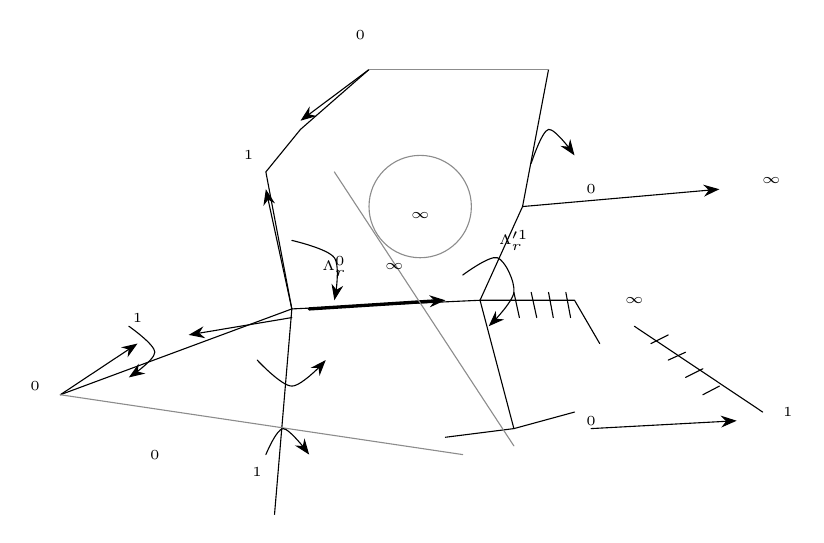
\begin{tikzpicture}[x=1mm,y=1mm,line cap=round,line join=round,font=\scriptsize]
\draw[pencil] (51.1,-26.1) circle[radius=6.5];
\node[inner sep=1pt] at (51.1,-27.2) {\tiny $\infty$};
\draw (34.8,-39.1) -- (31.5,-21.7) -- (35.9,-16.3) -- (44.6,-8.7);
\draw (34.8,-39.1) -- (5.4,-50);
\draw (34.8,-39.1) -- (32.6,-65.2);
\draw (34.8,-39.1) -- (58.7,-38) -- (70.7,-38) -- (73.9,-43.5);
\draw (58.7,-38) -- (64.1,-26.1) -- (67.4,-8.7);
\draw (58.7,-38) -- (63,-54.3) -- (54.3,-55.4);
\draw (63,-54.3) -- (70.7,-52.2);
\draw[-{Stealth[length=2mm]}] (64.1,-26.1) -- (89.1,-23.9);
\draw[-{Stealth[length=2mm]}] (72.8,-54.3) -- (91.3,-53.3);
\draw (78.3,-41.3) -- (94.6,-52.2);
\draw[-{Stealth[length=2mm]}] (5.4,-50) -- (15.2,-43.5);
\draw[{Stealth[length=2mm]}-] (21.7,-42.4) -- (34.8,-40.2);
\draw[-{Stealth[length=2mm]},very thick] (37,-39.1) -- (54.3,-38);
\draw[-{Stealth[length=2mm]}] (44.6,-8.7) -- (35.9,-15.2);
\draw[-{Stealth[length=2mm]}] (34.8,-39.1) -- (31.5,-23.9);
\draw[pencil] (5.4,-50) -- (56.5,-57.6);
\draw[pencil] (44.6,-8.7) -- (67.4,-8.7);
\draw[pencil] (40.2,-21.7) -- (63,-56.5);
\draw[-{Stealth[length=2mm]}] plot[smooth, tension=0.55] coordinates {(34.8,-30.4) (40.2,-32.6) (40.2,-38)};
\draw[-{Stealth[length=2mm]}] plot[smooth, tension=0.55] coordinates {(56.5,-34.8) (60.9,-32.6) (63,-37) (59.8,-41.3)};
\draw[-{Stealth[length=2mm]}] plot[smooth, tension=0.55] coordinates {(30.4,-45.6) (34.8,-48.9) (39.1,-45.6)};
\draw[-{Stealth[length=2mm]}] plot[smooth, tension=0.55] coordinates {(31.5,-57.6) (33.7,-54.3) (37,-57.6)};
\draw[-{Stealth[length=2mm]}] plot[smooth, tension=0.55] coordinates {(14.1,-41.3) (17.4,-44.6) (14.1,-47.8)};
\draw[-{Stealth[length=2mm]}] plot[smooth, tension=0.55] coordinates {(65.2,-20.6) (67.4,-16.3) (70.7,-19.6)};
\draw (63,-37) -- (63.7,-40.2);
\draw (65.2,-37) -- (65.9,-40.2);
\draw (67.4,-37) -- (68,-40.2);
\draw (69.6,-37) -- (70.2,-40.2);
\draw (80.4,-43.5) -- (82.6,-42.4);
\draw (82.6,-45.6) -- (84.8,-44.6);
\draw (84.8,-47.8) -- (87,-46.7);
\draw (87,-50) -- (89.1,-48.9);
\node[inner sep=1pt] at (43.5,-4.3) {\tiny $0$};
\node[inner sep=1pt] at (29.3,-19.6) {\tiny $1$};
\node[inner sep=1pt] at (72.8,-23.9) {\tiny $0$};
\node[inner sep=1pt] at (95.7,-22.8) {\tiny $\infty$};
\node[inner sep=1pt] at (2.2,-48.9) {\tiny $0$};
\node[inner sep=1pt] at (15.2,-40.2) {\tiny $1$};
\node[inner sep=1pt] at (17.4,-57.6) {\tiny $0$};
\node[inner sep=1pt] at (30.4,-59.8) {\tiny $1$};
\node[inner sep=1pt] at (72.8,-53.3) {\tiny $0$};
\node[inner sep=1pt] at (97.8,-52.2) {\tiny $1$};
\node[inner sep=1pt] at (78.3,-38) {\tiny $\infty$};
\node[inner sep=1pt] at (40.2,-33.7) {\tiny $\Lambda^0_r$};
\node[inner sep=1pt] at (63,-30.4) {\tiny $\Lambda'^1_r$};
\node[inner sep=1pt] at (47.8,-33.7) {\tiny $\infty$};
\end{tikzpicture}
\end{document}
